\section{Model-based Efficient Reasoning}

From the model perspective, these works focus on fine-tuning LLMs to improve their intrinsic ability to reason concisely and efficiently.

\subsection{RL with Length Reward Design}
\label{sec:rl}

Most reasoning models are trained using RL-based methods (e.g., DeepSeek-R1~\cite{guo2025deepseek}, DeepSeek-R1-Zero~\cite{guo2025deepseek}, OpenAI o1~\cite{openai_learning_to_reason}, QwQ-32B-Preview~\cite{qwen_qwq_32b_preview}) which focus on the accuracy reward and format rewards~\cite{guo2025deepseek}. To enhance reasoning-length efficiency, some studies propose integrating a length reward into the RL framework, which effectively shortens the reasoning process (as shown in Table~\ref{fig:rl}). In principle, the length reward assigns higher scores to short, correct answers while penalizing lengthy or incorrect ones, thereby optimizing the length of the reasoning path.

\begin{table}[t]
\centering
\small
\caption{Comparison of different length reward-based RL methods. $L(\cdot)$ denotes the way of calculating the prediction length. $r_0^c/r_0^w$ denotes reward (correct/wrong) for $L(\cdot)$=0. $r_L^c/r_L^w$ Reward (correct/wrong) for $L(\cdot) = L_\text{max}(\cdot)$. $r_e$ is the exceed length penalty. $y_\text{GT}$ represents the ground truth answer of input data $x$. $\pi_{\text{ref}}$ is the policy of reference model.}
\label{tab:rl-length}
\resizebox{\textwidth}{!}{
\begin{tabular}{l|c|c|c|c}
\toprule
\textbf{Method} & \textbf{RL} &  \textbf{Length Constraint Reward} & \textbf{Data} & \textbf{Model} \\
\midrule\midrule
O1-Pruner~\cite{luo2025o1} & PPO & $\mathbb{E}_{x \sim D} \left[ \mathbb{E}_{\pi_\theta, \pi_{\text{ref}}}\left[\frac{L(y_\text{ref})}{L(y_\text{pred})}\right] - 1 \right]
$ & \makecell[c]{GSM8K \\ GaoKao \\ MATH-500 } & \makecell[c]{Marco-o1-7B \\ QwQ-32B-Preview} \\
\midrule 
% KIMI~\cite{team2025kimi} & PPO & $\begin{cases}
%             \; \lambda & \!\text{if correct}, \lambda = 0.5\!-\!\frac{L(y_\text{pred})-L_{\min}}{L_{\max}- L_{\min}}\\
%             \; \min(0, \lambda) & \!\text{if wrong}.
%         \end{cases}$ & -- & -- \\
% \midrule 
Demystifying~\cite{yeo2025demystifying} & PPO & $\begin{cases}
            \; r_0^c + 0.5 \times (r_L^c - r_0^c)(1 + \cos({\frac{\pi L(y_\text{pred})}{L_{\max}}}), & \text{if correct}, \\
            \; r_0^c + 0.5 \times (r_L^w - r_0^w)(1 + \cos({\frac{\pi L(y_\text{pred})}{L_{\max}}}), & \text{if wrong} \\
            \; r_e, & \text{if } L(y_\text{pred}) = L_{\max},\end{cases}$
        & \makecell[c]{MATH-500 \\ AIME-2024 \\ TheoremQA \\  MMLU-Pro-1k } & \makecell[c]{LLaMA-3.1-8B \\ Qwen2.5-7B-Math} \\
\midrule
L1~\cite{aggarwal2025l1} & GRPO & $\begin{cases}
            \; x_\text{new} = \textit{CONCAT}~(x,\textit{“Think for N tokens.”}),\\
            \; r(y, y_{GT}, L(y_{GT})) = \mathbb{I}(y_\text{pred} =  y_{GT}) - \alpha \cdot |L(y_{GT}) - L(y_\text{pred})|
        \end{cases}$ 
       & \makecell[c]{AMC \\ GPQA \\ LAST \\ MMLU \\ MATH-500 \\ AIME-2024 \\ Olympiad-Bench  } & DeepSeek-R1-Distill-Qwen-1.5B \\
\midrule
DAST~\cite{shen2025dast} & SimPO & \makecell[c]{Trained with constructed length preference data} &  \makecell[c]{MATH-500 \\ AIME-2024} & \makecell[c]{DeepSeek-R1-Distill-Qwen-8B \\ DeepSeek-R1-Distill-Qwen-32B} \\
\midrule 
Training~\cite{arora2025training} & PG & $\mathbb{E}_{x \sim D}\left[ \mathbf{1}\{y_\text{pred} = y_\text{GT}\}(1 - \alpha f(L(y_\text{pred}))) \right]$ & \makecell[c]{GSM8K \\ MATH-500 \\ AIME-2024  } & \makecell[c]{DeepSeek-R1-Distill-Qwen-1.5B \\ DeepSeek-R1-Distill-Qwen-7B} \\
\bottomrule 
\end{tabular}
}
\end{table}

\begin{table}[t]
\centering
\small
\caption{Comparison of different policy optimization methods in CoT length controls. $\hat{R}_t$ represents the reward model. $\pi_{\text{ref}}$ is the policy of reference model. $\gamma$ is a target reward margin term for SimPO. $\lambda$ is a clipping-related hyper-parameter. The $y_w$ is for winning responses, and $y_l$ is for losing responses, where some with $G$ on superscript denote the outputs of different sampled groups.}
\label{tab:rl-comparison}
\scalebox{0.9}{
\begin{tabular}{l|c}
\toprule
\textbf{Method} & \textbf{Optimization Objective} \\
\midrule\midrule
Policy Gradient (PG) & $\mathbb{E}_{\pi_\theta}\left[ \nabla_\theta \log \pi_\theta(y_t|x_t) \hat{R}_t \right]$ \\
\midrule
PPO~\cite{schulman2017proximal} & $\mathbb{E}\left[ \min \Big( 
\frac{\pi_\theta(y_t  \mid x_t)}{\pi_{\theta_{\text{ref}}}(y_t  \mid x_t)}\hat{R}_t ,\ 
\text{clip}\left( 
\frac{\pi_\theta(y_t \mid x_t)}{\pi_{\theta_{\text{ref}}}(y_t \mid x_t)},\ 
1 - \epsilon,\ 
1 + \epsilon 
\right)\hat{R}_t  
\Big)
\right]$ \\
\midrule
SimPO~\cite{meng2024simpo} & $\mathbb{E}\left[ \log \sigma \left(
\frac{\beta}{|y_t^w|} \log \pi_\theta(y_t^w \mid x_t)
- \frac{\beta}{|y_t^l|} \log \pi_\theta(y_t^l \mid x_t)
- \gamma
\right) \right]$\\
\midrule
GRPO~\cite{shao2024deepseekmath} & $\mathbb{E}\left[ \min \Big( 
\frac{\pi_\theta(y^G_t  \mid x_t)}{\pi_{\theta_{\text{ref}}}(y^G_t  \mid x_t)}\hat{R}^G_t ,\ 
\text{clip}\left( 
\frac{\pi_\theta(y^G_t \mid x_t)}{\pi_{\theta_{\text{r}}}(y^G_t \mid x_t)},\ 
1 - \epsilon,\ 
1 + \epsilon 
\right)\hat{R}^G_t  
\Big) - \lambda\mathbb{D}_{KL}[\pi_\theta||\pi_{\text{ref}}] \right]$ \\
\bottomrule
\end{tabular}
}
\end{table}


\insightbox{The key question is: How to formulate the length reward in RL?}

\begin{figure}[h]
    \centering
    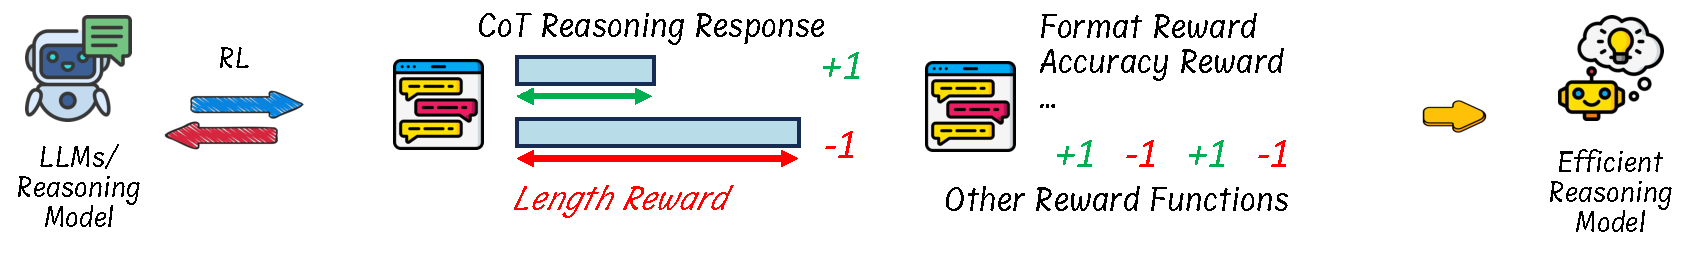
\includegraphics[width=\linewidth]{figs/rl.pdf}
    \caption{Illustration of the method for RL fine-tuning with length reward designs. In principle, the length reward assigns higher rewards to short, correct answers and penalizes lengthy or wrong answers to achieve efficient reasoning LLMs.}
    \label{fig:rl}
\end{figure}



Existing works leverage traditional RL optimization techniques combined with \textbf{\textit{explicit length-based reward}} to control the length of CoT reasoning. Some detailed length rewards are shown in Table~\ref{tab:rl-length}. 
The work~\cite{arora2025training} proposes utilizing length-based rewards conditioned on correctness, where shorter correct answers receive higher rewards. They then apply traditional policy gradient methods guided by this reward scheme to encourage LLMs to produce concise reasoning steps.
Expanding from the policy gradient, the following discussed work is primarily built upon proximal policy optimization (PPO)~\cite{schulman2017proximal} with CoT length penalty.
Demystifying~\cite{yeo2025demystifying} presents empirical findings from RL experiments examining how reasoning capability is influenced by length. They demonstrate that RL does not consistently or reliably increase the length and complexity of CoT reasoning, emphasizing the necessity of controlling CoT length growth to ensure stable performance. To mitigate these issues, they proposed a Cosine Reward based on a Dirichlet function of concise reward formula~\cite{loshchilov2016sgdr} and the proposed ``exceed length penalty'' scores.
Due to the performance impact of CoT length, Kimi k1.5~\cite{team2025kimi} incorporates a length penalty into its policy optimization (a variant of online policy mirror decent~\cite{tomar2020mirror}) to improve long CoT activations and facilitate effective model merging. Besides optimizing with length penalty reward, L1~\cite{aggarwal2025l1} modify the training data with the designated length constraint instruction (i.e., Think for $N$ tokens) before launching the policy optimization with pre-trained reasoning LLMs. 
O1-Pruner~\cite{luo2025o1} introduces the Length-Harmonizing Reward, combined with a PPO-style loss, to optimize reasoning LLMs by effectively shortening the CoT length. Specifically, the Length-Harmonizing Reward is computed based on the ratio of CoT lengths between the reference model output and the predicted results. Additionally, this reward incorporates accuracy-based constraints comparing predictions to the reference model outputs, ensuring that shortening the reasoning process does not degrade task performance.
Without relying on a reference model, DAST~\cite{shen2025dast} employs SimPO~\cite{meng2024simpo} to fine-tune reasoning LLMs using a constructed length-preference dataset. This dataset is generated based on a self-defined token-length budget measurement $L_\text{budget}$, defined as a linear combination of the average token length of correct responses and the maximum allowed generation length.

These RL-based methods enable the mitigation of overthinking in reasoning-capable LLMs, where overthinking refers to unnecessarily extended reasoning processes, leading to longer inference times and exceeding computational budgets. By achieving nearly lossless alignment with the original reasoning capabilities of LLMs, these budget-efficient RL strategies democratize the deployment of reasoning LLMs in resource-constrained scenarios.

